\documentclass{article}
\usepackage[utf8]{inputenc}
\usepackage{tikz}
\usetikzlibrary{shapes.geometric, arrows}

\tikzstyle{program} = [rectangle, rounded corners, minimum width=3cm, minimum height=1cm,text centered, draw=black, fill=red!30]
\tikzstyle{io} = [trapezium, trapezium left angle=70, trapezium right angle=110, minimum width=3cm, minimum height=1cm, text centered, draw=black, fill=blue!30]
\tikzstyle{process} = [rectangle, minimum width=3cm, minimum height=1cm, text centered, text width=3cm, draw=black, fill=orange!30]
\tikzstyle{decision} = [diamond, minimum width=3cm, minimum height=1cm, text centered, draw=black, fill=green!30]
\tikzstyle{arrow} = [thick,->,>=stealth]

\begin{document}

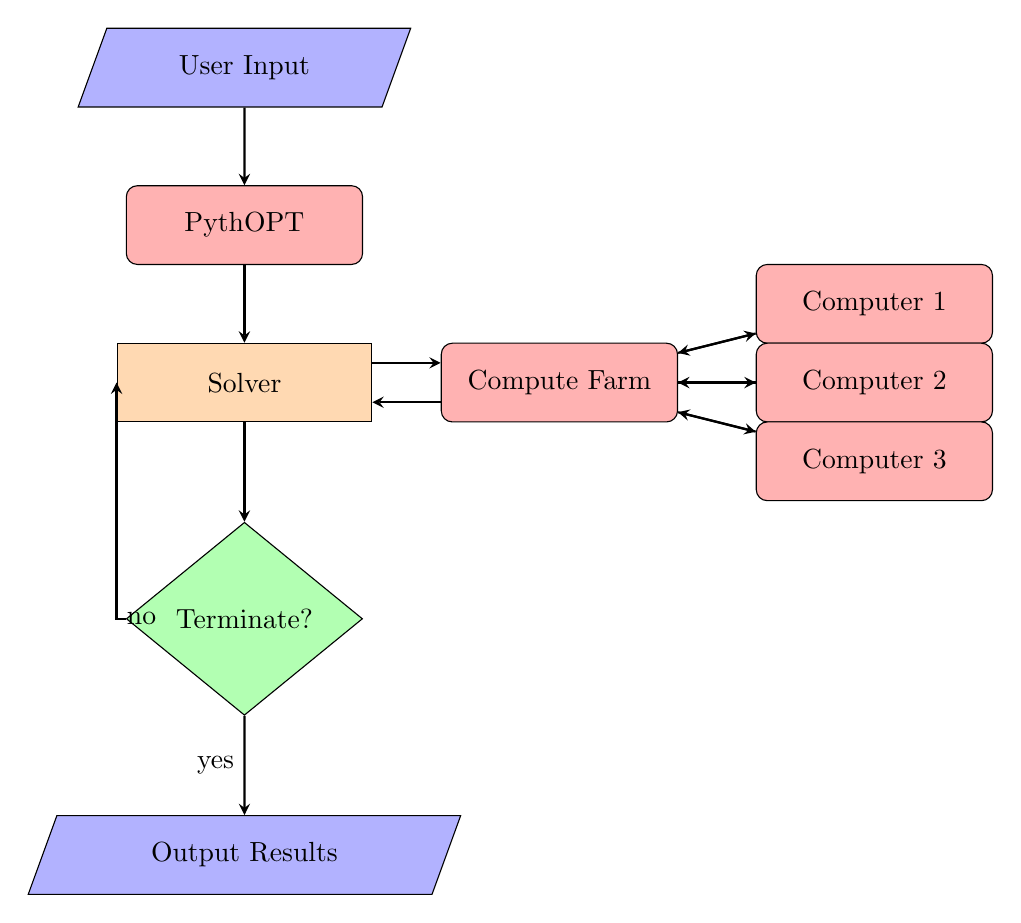
\begin{tikzpicture}[node distance=2cm]

\node (in1) [io] {User Input};
\node (pythopt) [program, below of=in1] {PythOPT};
\node (solver) [process, below of=pythopt] {Solver};
\node (compute) [program,right of=solver, xshift=2cm] {Compute Farm};
\node (dec) [decision, below of=solver,yshift=-1cm] {Terminate?};
\node (comp1) [program, right of=compute,yshift=1cm,xshift=2cm]  {Computer 1};
\node (comp2) [program, right of=compute,xshift=2cm] {Computer 2};
\node (comp3) [program, right of=compute,yshift=-1cm,xshift=2cm] {Computer 3};
\node (out1) [io, below of=dec,yshift=-1cm] {Output Results};


\draw [arrow] (in1) -- (pythopt);
\draw [arrow] (pythopt) -- (solver);
\draw [arrow,transform canvas={yshift=0.25cm}] (solver) -- (compute);
\draw [arrow,transform canvas={yshift=-0.25cm}] (compute) -- (solver);

\draw [arrow] (compute) -- (comp1);
\draw [arrow] (compute) -- (comp2);
\draw [arrow] (compute) -- (comp3);
\draw [arrow] (comp1) -- (compute);
\draw [arrow] (comp2) -- (compute);
\draw [arrow] (comp3) -- (compute);
\draw [arrow] (solver) -- (dec);
\draw [arrow] (dec) -- node[anchor=east] {yes} (out1);
\draw [arrow] (dec.west) -| node[anchor=west] {no} (solver.west);


\end{tikzpicture}

\end{document}

